% !TeX program = xelatex
\documentclass[10pt,a4paper]{ctexart} % 设置文章类型，正文字号与纸张大小

% 页面与正文常用宏包
\usepackage[margin=2cm]{geometry} % 设置页面四周页边距
\usepackage{graphicx}             % 插入图片
\usepackage{amsmath}              % 提供cases、aligned等数学公式环境
\usepackage{amssymb}              % 提供\therefore等扩展数学符号
\usepackage{booktabs}             % 提供\toprule、\midrule、\bottomrule三线表命令
\usepackage{float}                % 提供[H]固定图片、表格位置
\usepackage{subcaption}           % 提供subfigure子图环境及子图标题
\usepackage{wrapfig}              % 提供wrapfigure图文环绕环境
\usepackage{fancyhdr}             % 自定义页眉和页脚
\usepackage{hyperref}             % 生成超链接

% 页眉页脚
\pagestyle{fancy}                  % 启用fancyhdr定义的页面样式
\fancyhf{}                         % 清空默认页眉和页脚
\fancyfoot[C]{\thepage}            % 在页脚中央显示页码
\renewcommand{\headrulewidth}{0pt} % 隐藏页眉横线
\renewcommand{\footrulewidth}{0pt} % 隐藏页脚横线

% 超链接
\hypersetup{
  colorlinks=true,                % 使用彩色文字链接，而非带边框的链接
  linkcolor=red,                 % 目录、公式及图表交叉引用的颜色
  filecolor=cyan,                 % 本地文件链接的颜色
  urlcolor=blue,                  % 网址链接的颜色
  pdftitle={迈克尔逊干涉仪的应用预习报告},     % 写入PDF文档属性的标题
  bookmarksnumbered=true          % PDF书签显示章节编号
}

% 定义字号命令
\newcommand{\chuhao}{\fontsize{42pt}{63pt}\selectfont}
\newcommand{\xiaochu}{\fontsize{36pt}{54pt}\selectfont}
\newcommand{\yihao}{\fontsize{26pt}{39pt}\selectfont}
\newcommand{\xiaoyi}{\fontsize{24pt}{36pt}\selectfont}
\newcommand{\erhao}{\fontsize{22pt}{33pt}\selectfont}
\newcommand{\xiaoer}{\fontsize{18pt}{27pt}\selectfont}
\newcommand{\sanhao}{\fontsize{16pt}{24pt}\selectfont}
\newcommand{\xiaosan}{\fontsize{15pt}{22.5pt}\selectfont}
\newcommand{\sihao}{\fontsize{14pt}{21pt}\selectfont}
\newcommand{\xiaosi}{\fontsize{12pt}{18pt}\selectfont}
\newcommand{\wuhao}{\fontsize{10.5pt}{15.75pt}\selectfont}
\newcommand{\xiaowu}{\fontsize{9pt}{13.5pt}\selectfont}

% 章节格式
\ctexset{
  section={
    format={\CJKfontspec[AutoFakeBold=2.5]{KaiTi}\sanhao\bfseries}, % 一级标题使用三号加粗楷体
    name={,、},                                                    % 在中文章节序号后添加顿号
    number=\chinese{section},                                      % 一级标题编号使用“一、二、三”形式
    aftername={}                                                   % 取消编号与标题文字之间的空格
  },
  subsection={
    format={\CJKfontspec[AutoFakeBold=2.5]{KaiTi}\sihao\bfseries}, % 二级标题使用四号加粗楷体
  },
  subsubsection={
    format={\CJKfontspec[AutoFakeBold=2.5]{KaiTi}\xiaosi\bfseries}, % 三级标题使用小四加粗楷体
  }
}

\begin{document}

% 封面
\thispagestyle{fancy} % 封面保留底部居中的页码
\fancyfoot[C]{\thepage}
\begin{center}
  \CJKfontspec[AutoFakeBold=2.5]{KaiTi}\bfseries % 封面中文使用楷体并人工加粗，西文同时加粗
  \vspace*{2.0cm}
  \xiaochu 
    物理实验预习报告

  \vspace{3.8cm}
  \begin{minipage}{10.0cm}
    \sanhao
    \makebox[2.6cm][l]{实验名称：}
    \underline{\makebox[7.0cm][c]{迈克尔逊干涉仪的应用}}\par\vspace{12pt}

    \makebox[2.6cm][l]{指导老师：}
    \underline{\makebox[7.0cm][c]{包泽杭}}\par\vspace{12pt}
  \end{minipage}

  \vspace{3.8cm}
  \begin{minipage}{10.0cm}
    \sihao
    \makebox[1.4cm][l]{班级：}
    \underline{\makebox[8.0cm][c]{信工2503}}\par\vspace{10pt}

    \makebox[1.4cm][l]{姓名：}
    \underline{\makebox[8.0cm][c]{陈源}}\par\vspace{10pt}

    \makebox[1.4cm][l]{学号：}
    \underline{\makebox[8.0cm][c]{3250103617}}
  \end{minipage}

  \vspace{1.8cm}
  \sihao
    实验日期：
    \underline{\makebox[0.7cm][c]{2026}}年
    \underline{\makebox[0.7cm][c]{11}}月
    \underline{\makebox[0.7cm][c]{25}}日
    星期\underline{\makebox[0.7cm][c]{三}}上午

  \vspace{0.7cm}
  \sihao 
    浙江大学物理实验教学中心
\end{center}

\newpage
\xiaosi\songti\mdseries % 后续正文统一使用小四不加粗的宋体

\section{预习报告（10分）}

  \subsection{实验综述（5分）}
  
    \subsubsection{凸透镜成像原理}
    两列光波要形成稳定的干涉条纹，需要满足以下相干条件：
    \begin{enumerate}
      \item 频率：\( f_1 = f_2 \)
      \item 振动方向：\( \vec{A}_1 \parallel \vec{A}_2 \)
      \item 相位差：\( \phi_1 - \phi_2 = \text{定值} \)
      \item 光程差远小于相干长度
    \end{enumerate}

    满足这些条件后，可以根据相位差或光程差判断干涉结果：
    \[
    \begin{aligned}
        \text{干涉加强：}\quad
        & \phi_1 - \phi_2 = 2k\pi, \\
        & \delta = k\lambda,
          \quad k = 0, \pm 1, \pm 2, \ldots \\[1em]
        \text{干涉相消：}\quad
        & \phi_1 - \phi_2 = \pi + 2k\pi, \\
        & \delta = \frac{(2k+1)\lambda}{2},
          \quad k = 0, \pm 1, \pm 2, \ldots
    \end{aligned}
    \]

    \begin{figure}[H]
      \centering
      \begin{minipage}{0.3\textwidth}
        \centering
        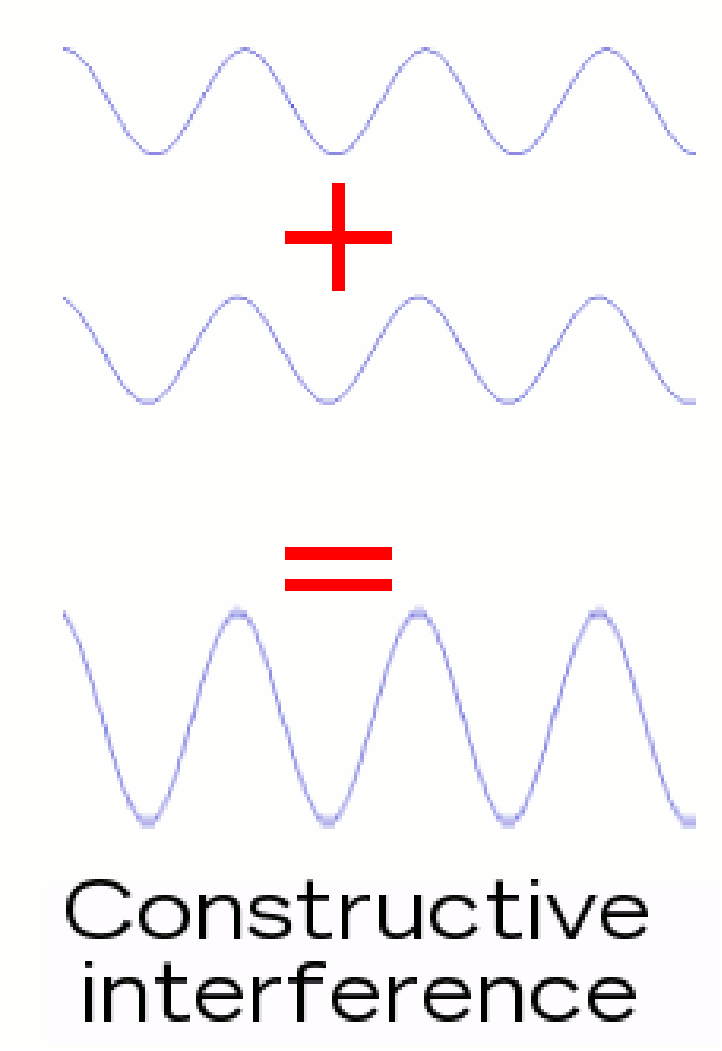
\includegraphics[width=\linewidth]{figures/图1.png}
        \caption{干涉加强}
      \end{minipage}
      \hfill
      \begin{minipage}{0.3\textwidth}
        \centering
        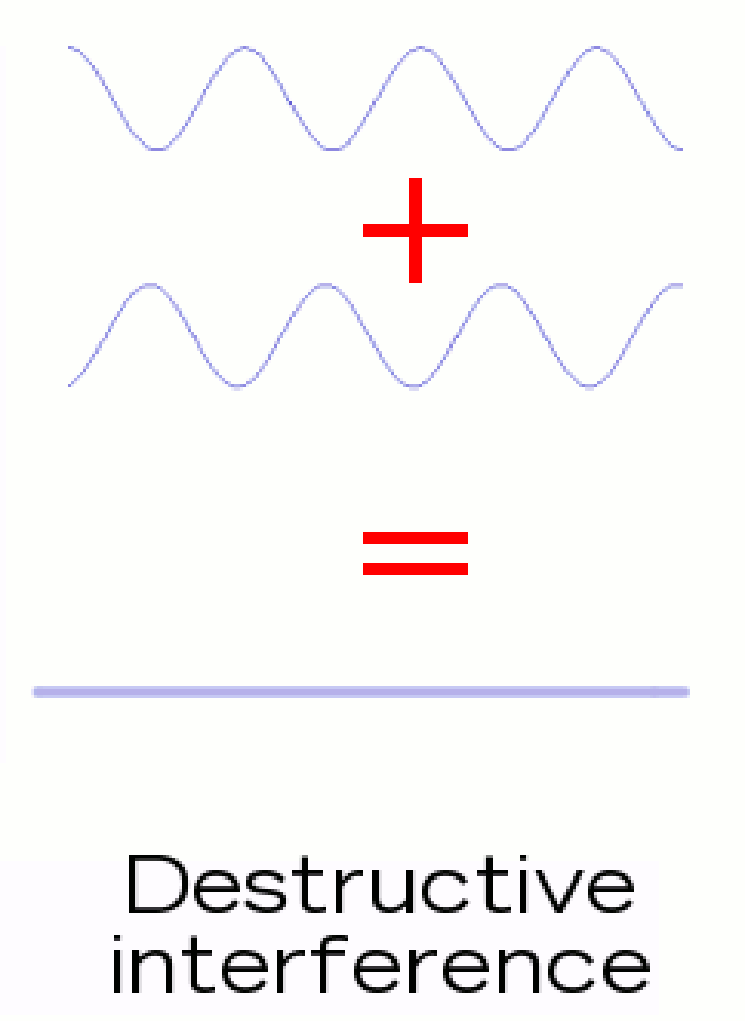
\includegraphics[width=\linewidth]{figures/图2.png}
        \caption{干涉相消}
      \end{minipage}
    \end{figure}

    \subsubsection{获取相干光的两种途径}
    为获得相干光，可以将同一光源发出的光分成两束，再使两束光重新相遇。
    \begin{itemize}
      \item 分波面法：点光源的波阵面分割为两部分，这两部分分别通过两个光具组，经反射、折射或衍射后交迭起来，在一定区域形成干涉。
      \item 分振幅法：当一束光投射到两种透明媒质的分界面上，光一部分反射，另一部分折射，若将它们再次汇聚后就会形成干涉。
    \end{itemize}

    \begin{figure}[H]
      \centering
      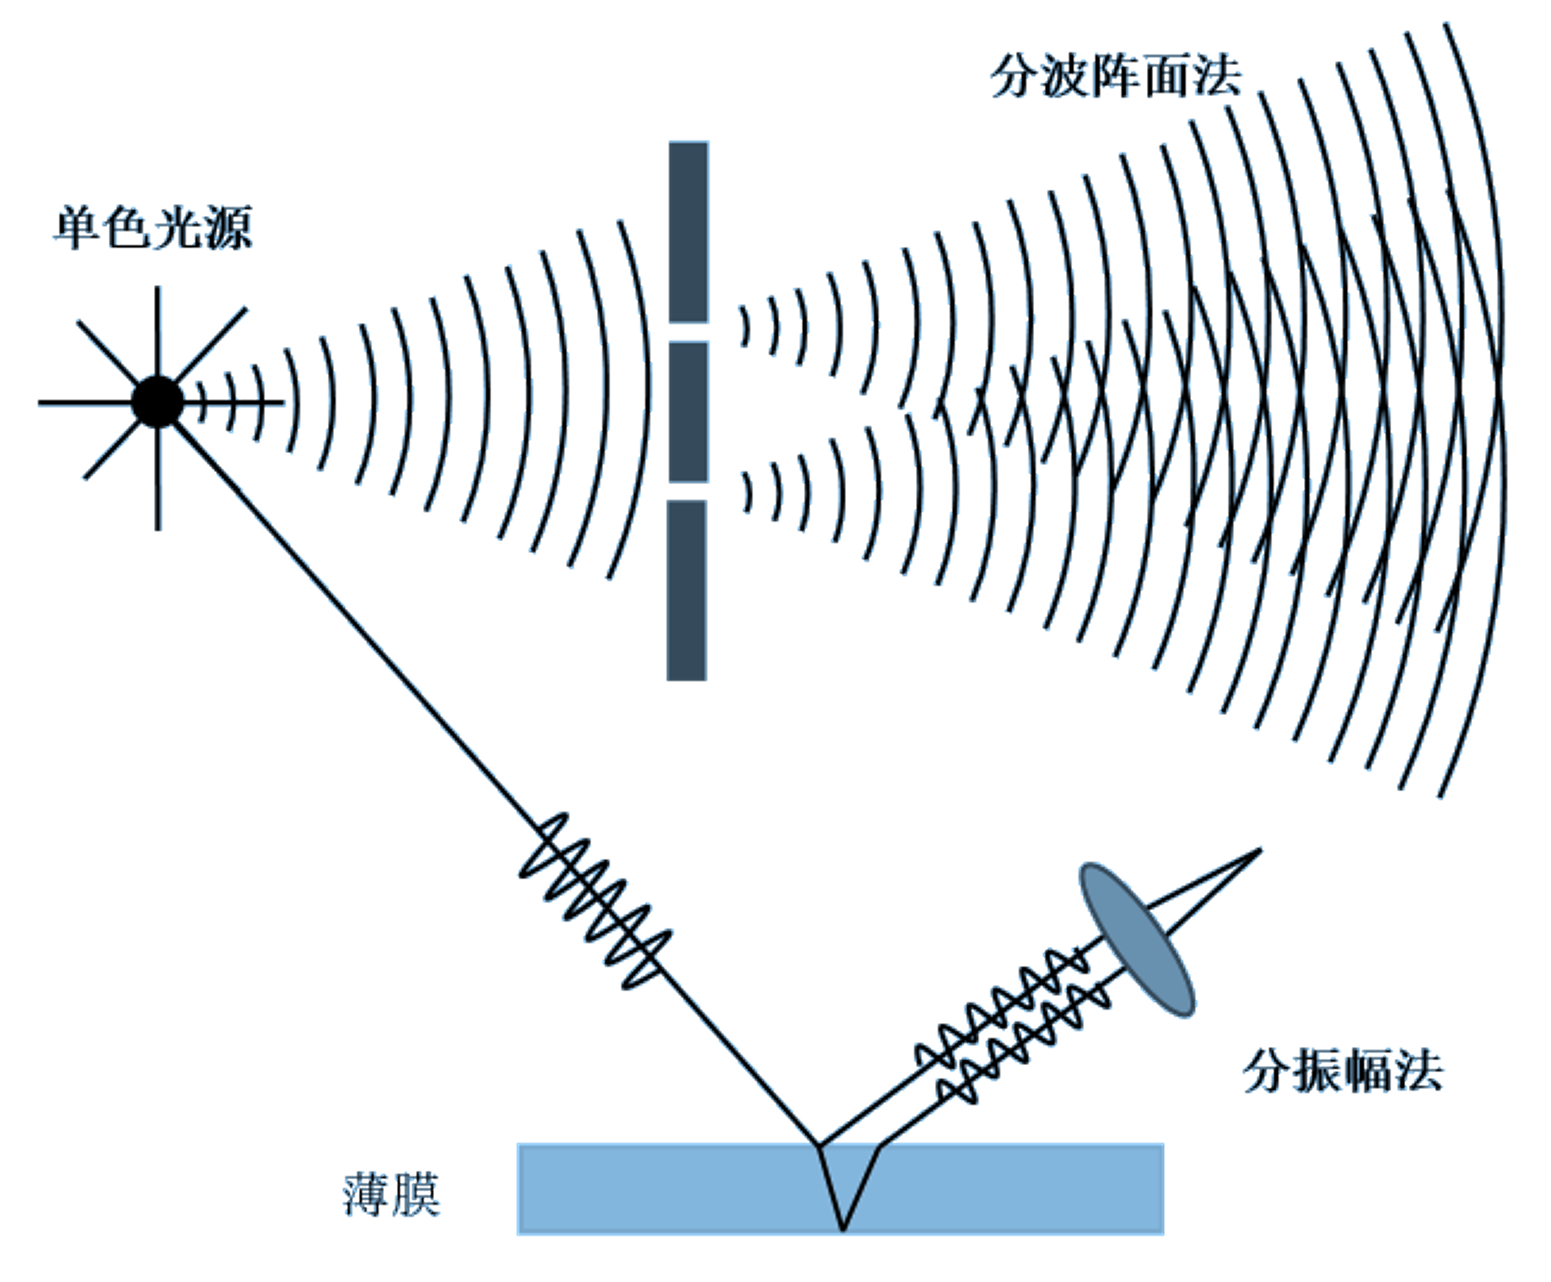
\includegraphics[width=0.45\textwidth]{figures/图3.png}
      \caption{获取相干光的两种途径}
    \end{figure}

    \subsubsection{迈克尔逊干涉仪光路图}

    迈克尔逊干涉仪利用分振幅法分出两束光，并使它们沿不同光路返回后汇合。
    \begin{itemize}
      \item 分光镜P1——利用分振幅法获得相干光。
      \item 补偿板P2——补偿分光镜因色散而产生的附加光程差；补偿相同入射角不同入射面光线所产生的附加光程差。
      \item 干涉现象——通过改变两光束夹角与光程差（移动镜距离，路径中折射率），探究多种干涉条纹。
    \end{itemize}

    \begin{figure}[H]
      \centering
      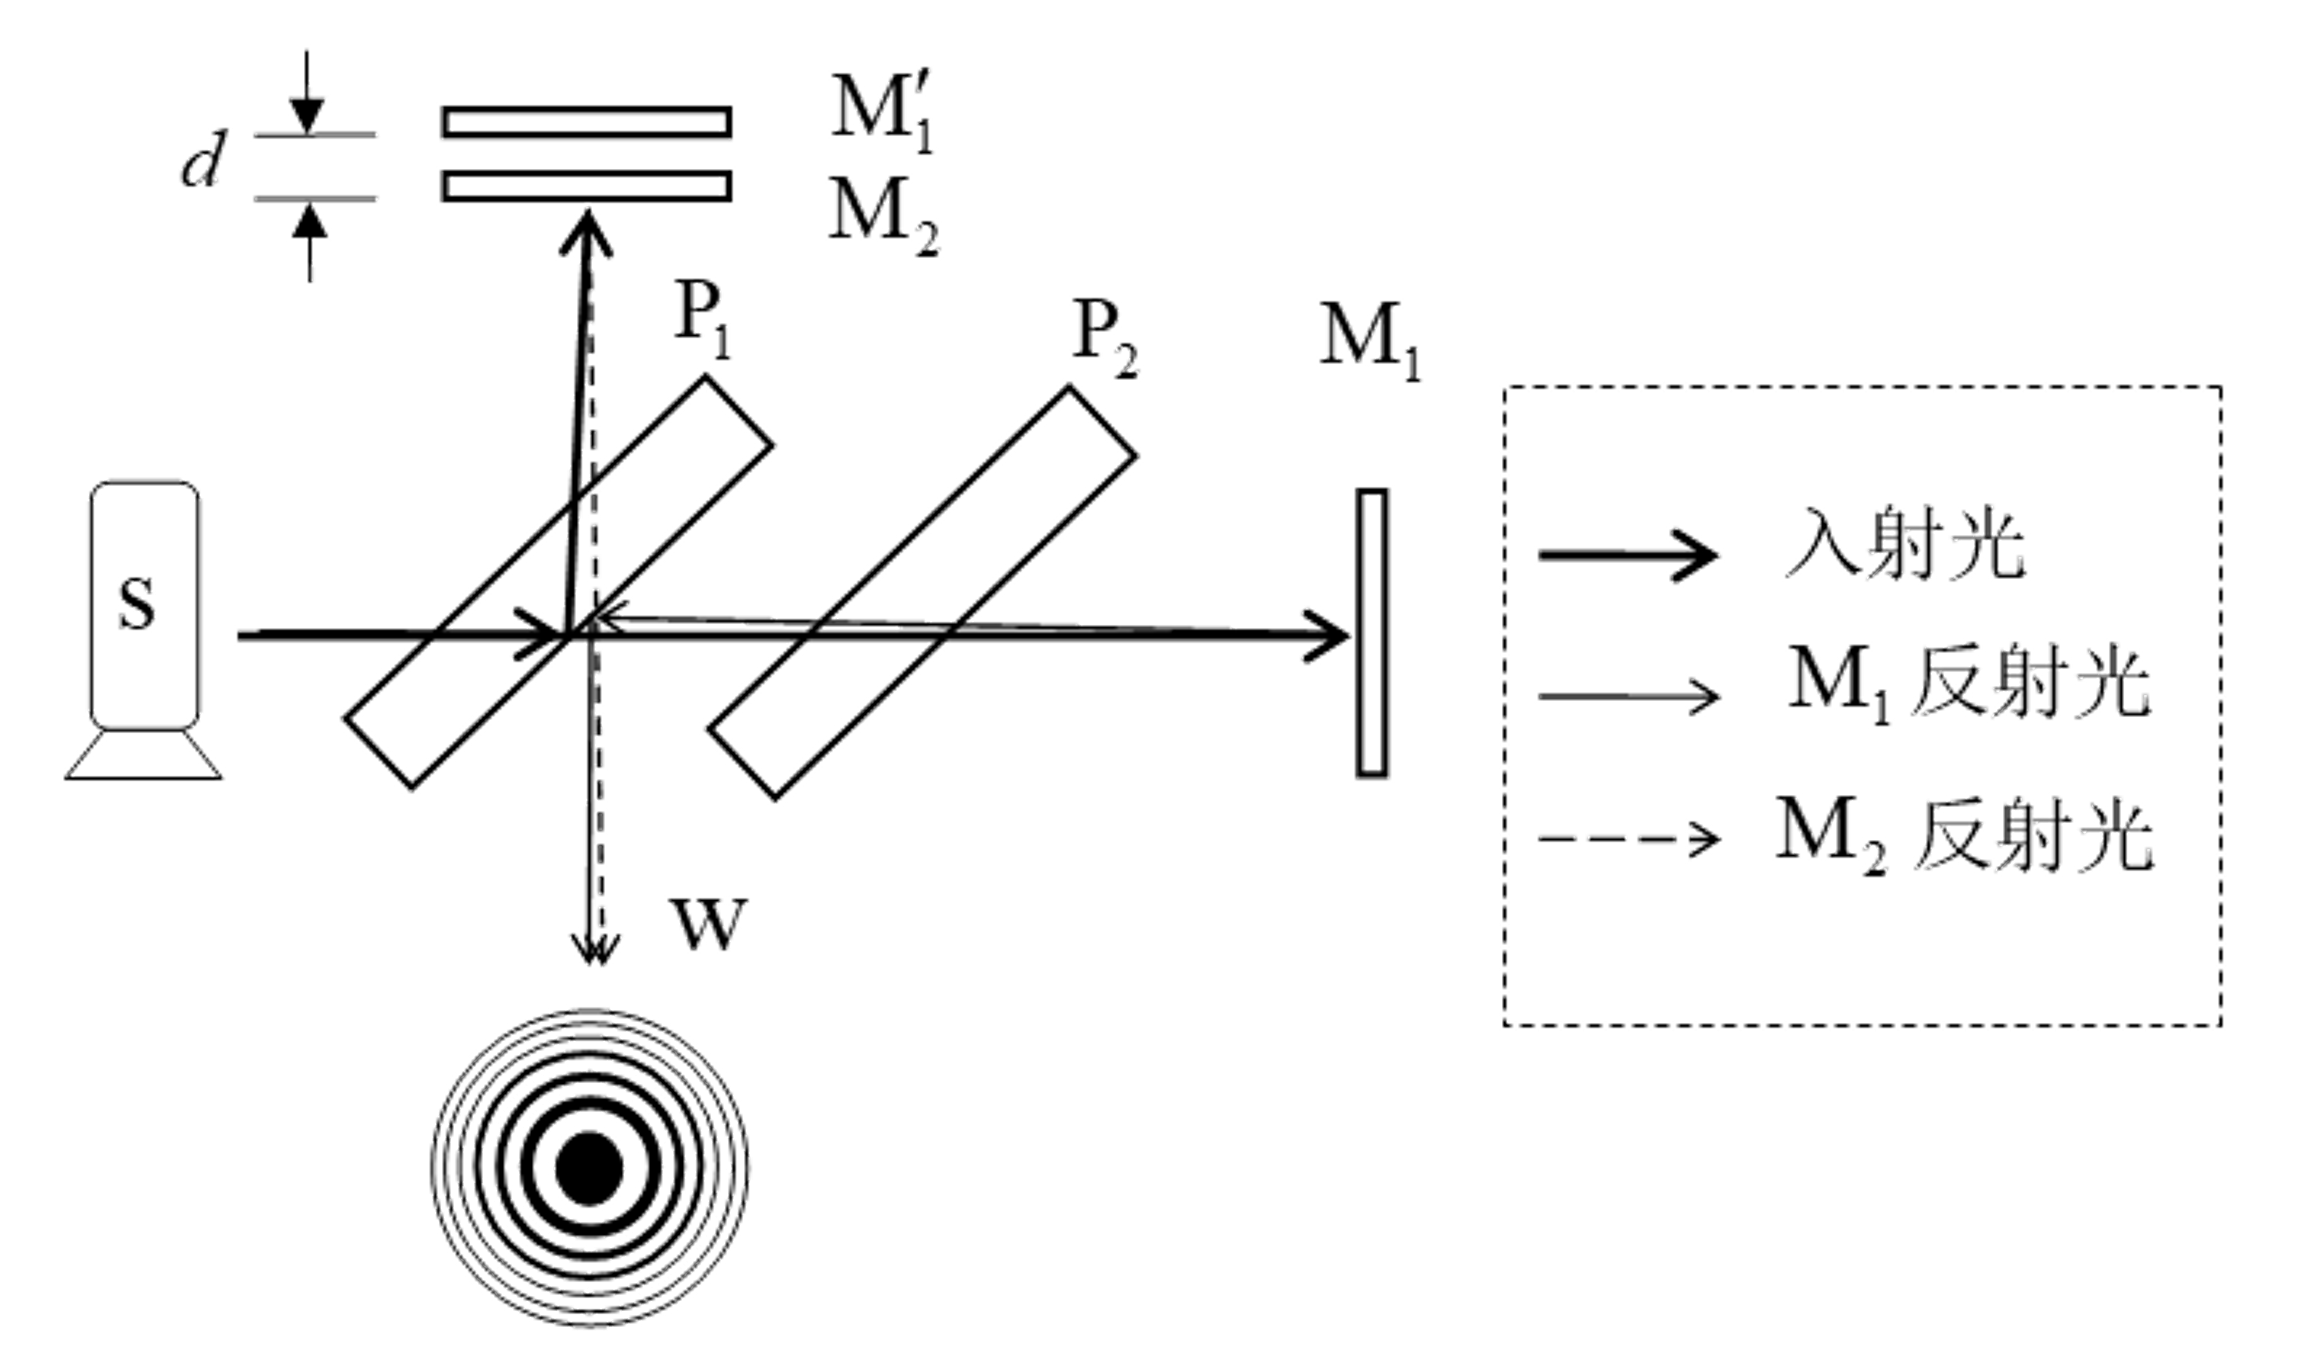
\includegraphics[width=0.5\textwidth]{figures/图4.png}
      \caption{迈克尔逊干涉仪光路图}
    \end{figure}

    \subsubsection{迈克尔逊定域等倾干涉}
    对于沿不同方向出射的光线，可以由光程差确定相应的干涉条件。
    两列相干光波的光程差为：
    \[
    \begin{aligned}
    \delta &= (AC + BC) - AD \\
          &= \frac{2d}{\cos\theta} - 2d\tan\theta\sin\theta \\
          &= 2d\cos\theta
    \end{aligned}
    \]

    对于第\(k\)级亮条纹，有：
    \[
    2d\cos\theta_k = k\lambda,
    \qquad k = 0, \pm 1, \pm 2, \pm 3, \ldots
    \]

    \begin{figure}[H]
      \centering
      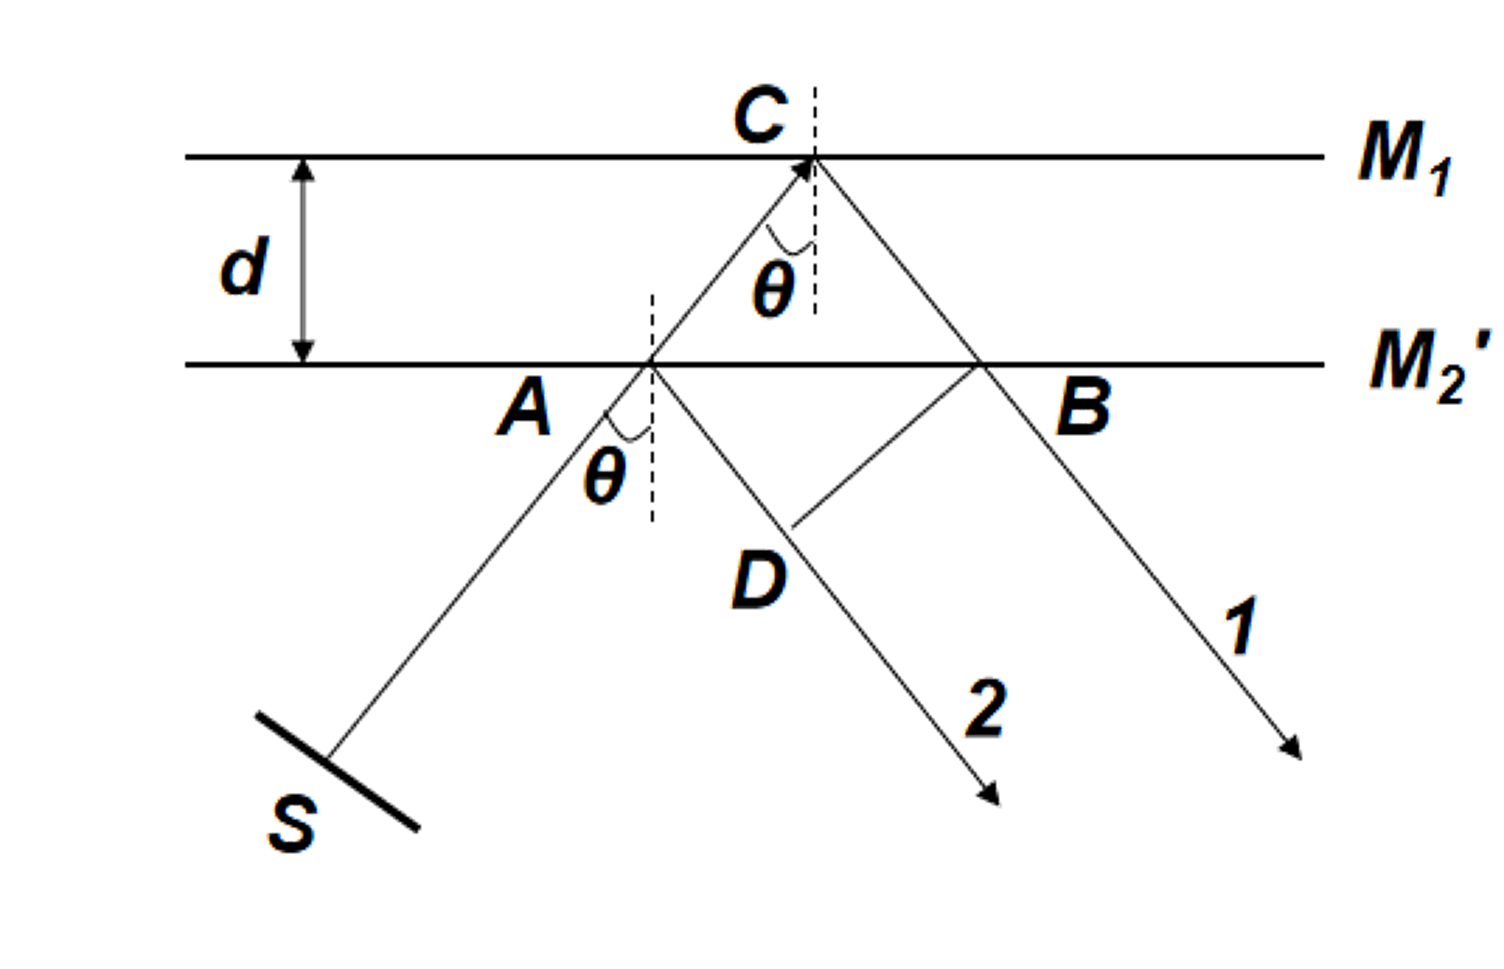
\includegraphics[width=0.4\textwidth]{figures/图5.png}
      \caption{迈克尔逊定域等倾干涉}
    \end{figure}

    \subsubsection{钠光波长的测定}
    在圆环中心，利用光程差与干涉级次的关系，可把环纹变化转化为波长测量。
    中心处光程差公式：
    \[
    2d = k\lambda,
    \qquad k = 0, \pm 1, \pm 2, \pm 3, \ldots
    \]

    中心吞吐\(N\)个环纹，光程差改变为：
    \[
    \Delta L = 2\Delta d = \Delta k\lambda = N\lambda
    \]

    波长测量公式：
    \[
    \boxed{\lambda = \frac{2\Delta d}{N}}
    \]

    \subsubsection{钠黄双线波长差的测定}
    两条波长接近的谱线形成的干涉条纹叠加后，条纹可见度随光程差变化。
    钠黄双线：
    \[
    \lambda_1 = 589.0\,\mathrm{nm},
    \qquad
    \lambda_2 = 589.6\,\mathrm{nm}
    \]

    条纹可见度最小：
    \[
    \Delta = k_2\lambda_2
    = \left(k_1+\frac{1}{2}\right)\lambda_1,
    \qquad
    k_1,\;k_2\text{ 为正整数}
    \]

    条纹可见度再次最小：
    \[
    \Delta+\Delta L
    = (k_2+k)\lambda_2
    = \left(k_1+k+1+\frac{1}{2}\right)\lambda_1
    \]

    \[
    \Delta L=\frac{\bar{\lambda}^{\,2}}{\Delta\lambda}
    \]

    双线波长差测量公式：
    \[
    \boxed{
    \Delta\lambda
    =\frac{\bar{\lambda}^{\,2}}{\Delta L}
    =\frac{\bar{\lambda}^{\,2}}{2\Delta d}
    }
    \]

    \begin{figure}[H]
      \centering
      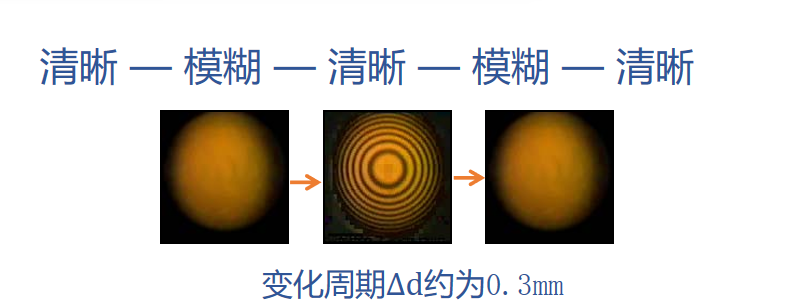
\includegraphics[width=0.4\textwidth]{figures/图6.png}
      \caption{钠黄双线波长差的测定}
    \end{figure}

    \subsubsection{实验内容}
    实验包括两项内容：测量钠光波长与钠黄双线波长差的测定。
    两项测量均需先调出清晰的圆环条纹，再根据条纹变化记录动镜位置。
    \begin{itemize}
      \item 测量钠光波长：等倾干涉条纹调出后，将CCD移到眼睛位置代替人眼，顺时针（或逆时针）转动微调手轮，
      观察干涉圆环形纹的“涌出”或“陷入”现象。待干涉圆环形纹的“涌出”或“陷入”现象正常后，
      继续同方向转动微调手轮观察并记录每“涌出”或“陷入”50个干涉圆环形条纹时， 动镜前后移动位置，计算钠光波长。

      \item 钠黄双线波长差的测定:
      \begin{enumerate}
        \item 转动粗调手轮，使条纹清晰可见（高对比度）。
        \item 在干涉圆环形条纹能正常“涌出”（或“陷入”）的前提下，记录$M_2$镜的初始位置，然后继续单向转动微调手轮，
        每当条纹对比度达到最低（几乎消失） 时，记录$M_2$镜位置的读数，连续测量3次以上。
        \item 依据测量得到的数据，根据公式，计算钠双线波长差。
      \end{enumerate}
    \end{itemize} 

  \subsection{实验重点（3分）}
  \begin{enumerate}
    \item 了解迈克尔逊干涉仪的结构并掌握调节方法；
    \item 观察光波干涉现象，加深对干涉理论的理解；
    \item 理解定域干涉与非定域干涉；
    \item 测量钠光波波长。
  \end{enumerate}

  \subsection{实验难点（2分）}
  \begin{enumerate}
    \item 调节光路，使两束光重合并获得清晰、稳定的圆环条纹；
    \item 准确计数中心环纹的涌出或陷入，并读取动镜位移以测定钠光波长；
    \item 判断条纹可见度最小的位置，测定钠黄双线的波长差。
  \end{enumerate}

\vspace*{\fill} % 使下面内容在页面底部显示
\noindent
\begin{minipage}{\textwidth}
  注意事项：

  \begingroup
    \setlength{\leftskip}{2em} % 1--4整体向右缩进两个汉字宽度
    1. 用PDF格式上传“实验报告”，文件名：学生姓名+学号+实验名称+周次。

    2. “实验报告”必须递交在“学在浙大”本课程内对应实验项目的“作业”模块内。

    3. “实验报告”成绩必须在“浙江大学物理实验教学中心网站”-“选课系统”内查询。

    4. 教学评价必须在“浙江大学物理实验教学中心网站”-“选课系统”内进行，学生必须进行教学评价，才能看到实验报告成绩，教学评价须在本次实验结束之后3天内进行。\par
  \endgroup

  \begin{center}
    {\CJKfontspec[AutoFakeBold=2.5]{SimSun}\bfseries 浙江大学物理实验教学中心制}
  \end{center}
\end{minipage}

\end{document}

